% --------------------------------------------------------------------------- %
% Warwick poster template created by Samuel Maloney, May 2021
% Updated January, 2024
%
% The brand colours have been updated to the latest on the website.
% The logo header, however is from the previous brand iteration's abstract
% poster template.
% --------------------------------------------------------------------------- %
\RequirePackage{silence}
\WarningFilter{pgf}{Snakes have been superseded by decorations}
\documentclass[latin,a0paper,portrait]{xebaposter}
\usepackage{uwposter}


\usepackage{algorithm}
\usepackage[noend]{algpseudocode}

%%%%% Items related to the Bibliography %%%%%%%%%%%%%%%%%%%%%%%%%%%%%%%%%%%%%%%
% The bibliography style can be set here. See available styles at:
% https://www.overleaf.com/learn/latex/Biblatex_bibliography_styles
\usepackage[backend=bibtex,style=chem-rsc,maxnames=2,minnames=2]{biblatex}
% This package provides (relatively) automatic journal name abbreviations.
% https://github.com/compholio/jabbrv
\usepackage[warnundef]{jabbrv}
% Add .bib file
\addbibresource{References.bib}

%%% Global Settings %%%%%%%%%%%%%%%%%%%%%%%%%%%%%%%%%%%%%%%%%%%%%%%%%%%%%%%%%%%
% \graphicspath{{fig/}}	% Root directory for graphics includes
% \tracingstats=2       % Enabled LaTeX logging with conditionals

%%%%%%%%%%%%%%%%%%%%%%%%%%%%%%%%%%%%%%%%%%%%%%%%%%%%%%%%%%%%%%%%%%%%%%%%%%%%%%%%
%%% Utility functions %%%%%%%%%%%%%%%%%%%%%%%%%%%%%%%%%%%%%%%%%%%%%%%%%%%%%%%%%%

%%% Save space in lists. Use this after the opening of the list
% \newcommand{\compresslist}{
% 	\setlength{\itemsep}{1pt}
% 	\setlength{\parskip}{0pt}
% 	\setlength{\parsep}{0pt}
% }
%%% This is simpler if all lists 'compressed' (uses the enumitem package)
\setlist{itemsep=1pt,topsep=3pt,parsep=0pt,partopsep=0pt,leftmargin=1.5em}

\newcommand{\reducegap}{\vspace{-4pt}}

%%%%%%%%%%%%%%%%%%%%%%%%%%%%%%%%%%%%%%%%%%%%%%%%%%%%%%%%%%%%%%%%%%%%%%%%%%%%%%%
%%% Document Start %%%%%%%%%%%%%%%%%%%%%%%%%%%%%%%%%%%%%%%%%%%%%%%%%%%%%%%%%%%%
%%%%%%%%%%%%%%%%%%%%%%%%%%%%%%%%%%%%%%%%%%%%%%%%%%%%%%%%%%%%%%%%%%%%%%%%%%%%%%%

\begin{document}
\typeout{Poster rendering started}

%%% Setting Background Image %%%%%%%%%%%%%%%%%%%%%%%%%%%%%%%%%%%%%%%%%%%%%%%%%%
% Used only if background=user is set in poster options.
\background{
	\begin{tikzpicture}[remember picture,overlay]%
    \draw (current page.north west) node[anchor=north west, inner sep=0pt]
	    {\includegraphics[height=\paperheight,width=\paperwidth]{templateFiles/masterLogo.pdf}};
	\end{tikzpicture}
}

% Move title down if master logo header is used.
% (The header is added right at the end of this file.)
\addtolength{\topmargin}{0.7in}
\addtolength{\textheight}{-0.7in}

%%% General Poster Settings %%%%%%%%%%%%%%%%%%%%%%%%%%%%%%%%%%%%%%%%%%%%%%%%%%%
%%%%%% Eye Catcher, Title, Authors and University Images %%%%%%%%%%%%%%%%%%%%%%
\begin{poster}{
    grid=false, % Display a grid, which can be useful during the layout phase
    columns=2, % # of columns; default 4 in landscape, 3 in portrait; max 6
    % colspacing=, % Distance between columns
    headerheight=0.125\textheight, % Height of the main poster header (not the headers of the text boxes) as a length. Default is 0.1\textheight, I've set it larger for the master logo
    background=shadeTB,
    bgColorOne=white, % 1st background color
    bgColorTwo=BrightBlue, % 2nd background color
    headerColorOne=DarkBlue,
    % headerColorTwo=BrightBlue,
    eyecatcher=true, % set true to centre title, false for left-justified
    % borderColor=WarwickGrey,
    textborder=none,
    headerborder=none,
    % headershape=roundedright,
    headershade=plain,
    textfont=\color{WarwickGrey},
    boxshade=plain,
    headerfont=\Large\sffamily,
    headerFontColor=white,
    % linewidth=,
    boxColorOne=white
    % boxColorTwo=
}
%%% Eye Catcher %%%%%%%%%%%%%%%%%%%%%%%%%%%%%%%%%%%%%%%%%%%%%%%%%%%%%%%%%%%%%%%
{
	% Eye Catcher, if option eyecatcher=false then it is unused
	% If left empty with eyecatcher=true, then nothing is inserted, but the title is centred
}
%%% Title %%%%%%%%%%%%%%%%%%%%%%%%%%%%%%%%%%%%%%%%%%%%%%%%%%%%%%%%%%%%%%%%%%%%%
{
    \color{WarwickGrey}\sffamily\bfseries
	Exponential Integrators\vspace{6pt}\\
	for PDEs\vspace{10pt}
}
%%% Authors %%%%%%%%%%%%%%%%%%%%%%%%%%%%%%%%%%%%%%%%%%%%%%%%%%%%%%%%%%%%%%%%%%%
{
    % \begin{center}
    \color{WarwickGrey}
	\textbf{Harvey Sutton}, Andreas Dedner\\
	\vspace{-2pt}
	{\smaller[2] Mathematics Institute, University of Warwick, Coventry, UK}\\
	\vspace{2pt}
	{\smaller[2] harvey.sutton@warwick.ac.uk}
% 	\end{center}
}
%%% Logo %%%%%%%%%%%%%%%%%%%%%%%%%%%%%%%%%%%%%%%%%%%%%%%%%%%%%%%%%%%%%%%%%%%%%%
{
% Insert an invisible box where the logo is to correctly position the title
\hbox{\phantom{\rule{0.3\textwidth}{0.1\textheight}}}
% \hbox{\rule{0.3\textwidth}{0.1\textheight}} % make box visible for testing

% Can be used to insert the 3rd party logo.
% Should also then remove the master logo header from the end of this file
% and the margin adjustments before the start of the poster class.
% 
\includegraphics[height=7em]{templateFiles/3rdPartyLogo.pdf}
}

% This section shows the use of the 'span' parameter to give it multiple column width
\headerbox{Motivation}
{name=motivation,column=0,row=0,span=2}
{
\begin{multicols}{2}
\begin{itemize}
\item Solutions to PDEs are important across scientific disciplines 
\item One approach is to use exponential integrators
\item These methods can be computationally demanding as we need to calculate the matrix exponential $e^Av$ which can be expensive
\item Kyrlov subspace methods have recently gained traction for a way to compute the matrix exponential efficiently\cite{Moler2003}.
\end{itemize}
For a discretised PDE: $\dot u = N(u)$ with Forward Euler time-stepping we get: $u^{n+1} = u^n+\tau N(u^n)$ for $\tau < \tau_{FE}$ where $\tau_{FE}$ depends on the specific problem. Using exponential integrators we have $u^{n+1} = e^{DN(u^n)\tau}(u^n + \tau(N(u^n)-DN(u^n)))$ which, for some problems can work for $\tau >> \tau_{FE}$ reducing the number of steps neccessary.
\columnbreak

\begin{center}
    \includegraphics[width=0.5\linewidth,height=0.1\textheight]{FEPics/Parabolic Test2_10x10_0.0001_EXPARN_EndTime=0.02.png}
    \captionof{figure}{Parabolic Equation at $T=0.02$ Computed with the using the Arnodli method}
    \label{fig:example_a}
\end{center}

\end{multicols}
}


\headerbox{1) Algorithms}
{name=section_one,span=1,column=0,below=motivation}
{
We compare several algorithms for computing the matrix exponential:
\begin{itemize}
\item Arnoldi
\item Lanczos \cite{OJALVO1970}
\item Kiops \cite{Gaudreault2018}
\end{itemize}
\begin{center}
\begin{algorithm}[H]
\caption{Arnoldi \cite{Fan2018}} %find better citation
\begin{algorithmic}
\Procedure{Arnoldi}{$A, \hat v_1,m$}
\State $v_0 \gets 0$
\For{$j = 1,2,...,m$}	
\For{$i = 1,2,...,j$}
\State$h_{ij} \gets v_i^T A v_i$
\EndFor
\State$\theta_j \gets Av_j - \sum^j_{i=1} h_{ij}v_i$
\State$h_{j+1,j} \gets ||\theta_j||$
\State$v_{j+1} \gets \theta_j/h_{j+1,j}$
\EndFor
\EndProcedure
\end{algorithmic}
\end{algorithm}
\end{center}
}

% Using 'above=bottom' will stretch it vertically for an even bottom line on all columns
\headerbox{2) Results for Parabolic Equation}
{name=section_two,span=1,column=0,below=section_one,above=bottom}
{
Bellow we compare results for a parabolic equation with the true solution given by:
\begin{align*}
\text{with exact solution }\hat u(t,x) &= cos(4\pi t)cos(2\pi x_0)
\end{align*}
We compare the error relative to the true solution with the number of calls to the operator:
\begin{center}
    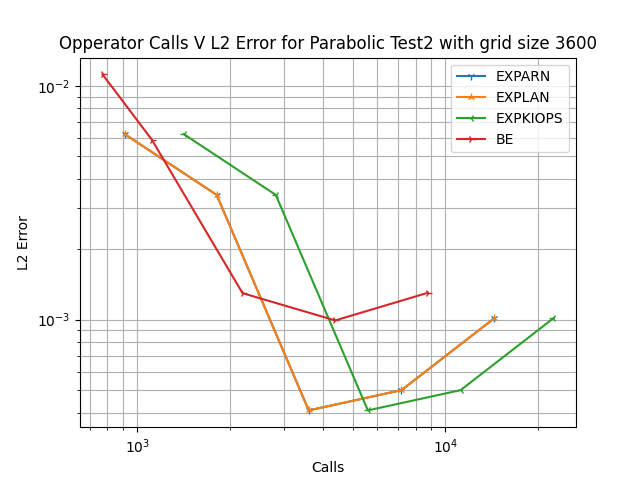
\includegraphics[width=0.8\linewidth,height=0.2\textheight]{FEMethodPlots/Operator Calls V Error for Parabolic Test2 with grid size 3600.png}
    \captionof{figure}{Comparision of Several Methods for a Parabolic Problem Note: The Arnoldi and Lanczos Methods performed identically}
    \label{fig:example_c}
\end{center}
From this and other results that have been omitted for brevity:
\begin{itemize}
\item The Kyrlov methods achieved a lower minimum bound
\item The difference between the Kyrlov methods and the Backwards Euler methods was more pronounced for larger grid sizes
\end{itemize}
}


\headerbox{3) Applications to Allen Cahn Equations}
{name=section_three,span=1,column=1,below=motivation}
{
Here we look at using these Kyrlov-based solvers to compute solutions for the Allen Cahn Equations:
\begin{figure}[H]
    \centering
    \begin{minipage}{0.49\textwidth}
	    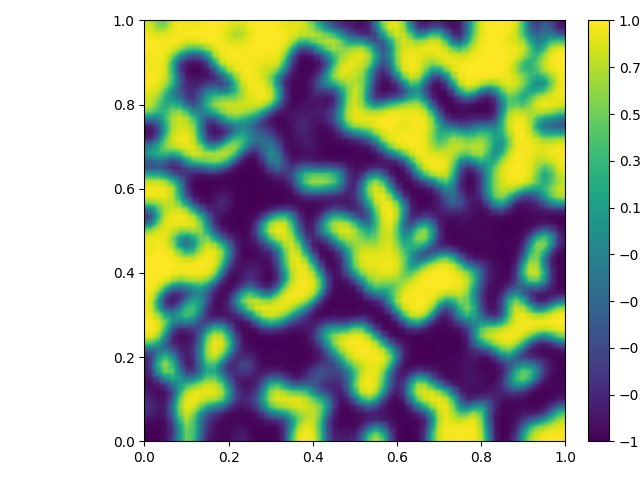
\includegraphics[width=1\linewidth,height=0.135\textheight]{FEPics/Allen Cahn Test2_60x60_0.025_Seed BE_EndTime=50.png}
	    \captionof{figure}{The Initial Condtion}
	    \label{fig:example}
    \end{minipage}\hfill
    \begin{minipage}{0.49\textwidth}
	\begin{center}
		The Allen Cahn equations in weak form are given by:
		\begin{align*}
		\int_{\Omega} \partial_tu v dx &= a(u,v)\\
		&\text {where }\\
		a(u,v) &= \int_{\Omega} 10^{-4} \nabla u \cdot \nabla v\\
			  &+ (u^2-1)uv dx
		\end{align*}
	\end{center}
    \end{minipage}\hfill
    \begin{minipage}{0.49\textwidth}
	    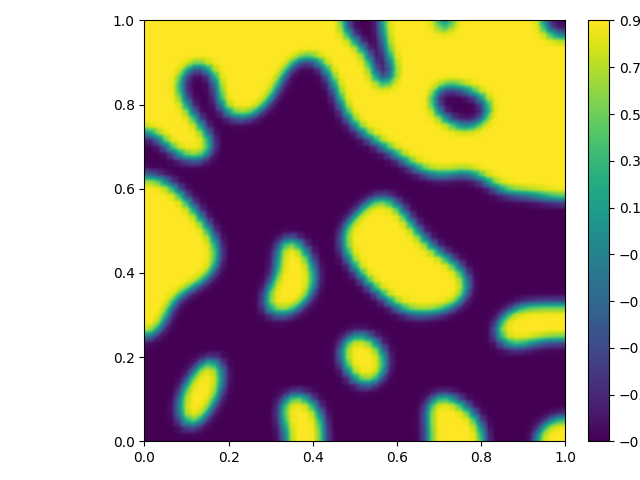
\includegraphics[width=1\linewidth,height=0.135\textheight]{FEPics/Allen Cahn Test2_60x60_0.025_EXPARN_EndTime=20.png}
	    \captionof{figure}{Allen Cahn Equation Solution Using the Arnoldi Algorithm at T=20}
	    \label{fig:example}    
    \end{minipage}\hfill
    \begin{minipage}{0.49\textwidth}
	    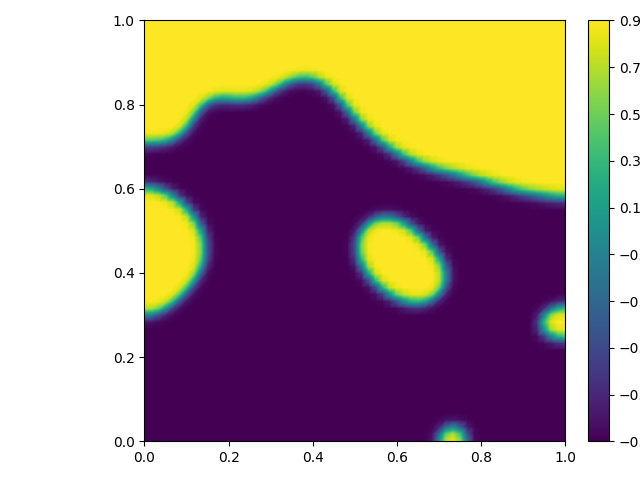
\includegraphics[width=1\linewidth,height=0.135\textheight]{FEPics/Allen Cahn Test2_60x60_0.025_EXPARN_EndTime=50.png}
	    \captionof{figure}{Allen Cahn Equation Solution Using the Arnoldi Algorithm at T=50}
	    \label{fig:example}
    \end{minipage}
\end{figure}
We observed that the different methods tested for the same initial conditions produced approximately the same results.
}


\headerbox{4) Concluding Remarks}
{name=section_four,span=1,column=1,below=section_three}
{
Conclusions:
\begin{itemize}
\item Kyrlov methods appear to outperform the Backwards Euler Method
\item These methods also seem effective for providing solutions to the Allen Cahn Equation
\end{itemize}
}


\headerbox{References and Acknowledgements}
{name=references,span=1,column=1,below=section_four,above=bottom}
{
\AtNextBibliography{\smaller} % Make the bibliography text smaller
\printbibliography[heading=none]
\reducegap
\reducegap
\smaller % Make the acknowledgement text smaller
Research supported by the Undergraduate Research Support Scheme from The University of Warwick.
}


\end{poster}
\begin{tikzpicture}[remember picture,overlay]%
    \draw (current page.north west) node[anchor=north west, inner sep=0pt]
	    {
\includegraphics[width=\paperwidth]{templateFiles/MasterLogo.png}};
\end{tikzpicture}
\end{document}